\chapter{Synchronizacja czasu}

Synchronizacja czasu jest jednym z podstawowych problemów systemów opartych o wiele urządzeń posiadających własne zegary. Wiedza o dokładnym czasie zachodzących w sieci zdarzeń jest niezbędna do szybkiego przesyłu danych, koordynacji procesów czy aktualizacji systemu plików. W przypadku niniejszej pracy dokładne określenie czasu zachodzących zdarzeń jest kluczowe do wiarygodnego określenia odległości pomiędzy węzłami na podstawie interwału czasowego pomiędzy nadaniem a odbiorem sygnału dźwiękowego.

\section{Synchronizacja programowa}

Pierwszym podejściem do rozwiązania problemu synchronizacji zegarów było zastosowanie synchronizacji programowej~\cite{6066334}, w której urządzenie-host utrzymuje wysokiej rozdzielczości licznik czasowy i wysyła sygnały o jego wartości pozostałym węzłom w sieci. Na podstawie tych informacji każdy z węzłów oblicza różnicę w zegarach i wprowadza odpowiednie przesunięcie własnego licznika.

\subsection{Algorytm synchronizacji NTP}

Jednym z najbardziej rozpowszechnionych protokołów synchronizacji programowej jest \textit{Network Time Protocol} opisany w pracy~\cite{103043}. Zachowując oznaczenia w niej zastosowane opiszmy w skrócie zasadę działania tego protokołu.

Na rysunku~\ref{fig:ntp} przestawiono schemat działania protokołu NTP. Urządzenia \textit{A} i \textit{B} wymieniają wiadomości zawierające sygnatury czasowe. Niech $T_{i},\ T_{i-1},\ T_{i-2},\ T_{i-3}$ będą czterema ostatnimi wiadomościami oraz niech $a = T_{i-2} - T_{i-3}$ oraz $b = T_{i-1} - T_i$. Wtedy całkowity czas transmisji $\delta_i$ i przesunięcie zegara $\theta_i$ urządzenia \textit{B} względem urządzenia \textit{A} to

\[\delta_i = a - b\quad \text{oraz}\quad \theta_i = \frac{a+b}{2}\]

Dodatkowym wnioskiem przedstawionym w powyższej pracy jest własność prawdziwego przesunięcia względem aktualnie obliczonego:

\[\theta_i - \frac{\delta_i}{2} \leq \theta \leq \theta_i + \frac{\delta_i}{2}\]

Jak łatwo zauważyć im krótszy jest czas propagacji tym lepsze przybliżenie dostajemy.

\begin{figure}
    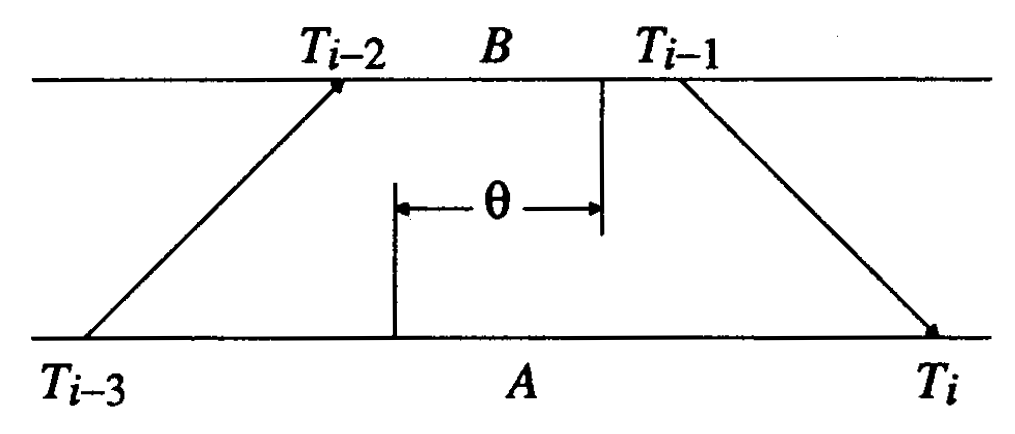
\includegraphics[width=\textwidth]{pics/ntp.png}
\caption{Pomiar opóźnienia transmisji i przesunięcia zegara}
\label{fig:ntp}
\end{figure}

Na postawie tych informacji podjęto próbę synchronizacji programowej zegarów węzłów w systemie multilateracyjnym.

\subsection{Pomiar różnic zegarów}



\section{Synchronizacja sprzętowa}

\subsection{Synchronizacja z użyciem mikrofonów}
